\chapter{具体需求}
\section{功能需求}

本章节描述xyz云盘系统所必须执行的基本动作,以及其输入、输出,以及中间处理的过程。

% 用户相关

\subsection{R.XYZ.CLOUDSTORAGE.USER.LOGIN.001 用户:显示初始登陆界面 }

\subsubsection{介绍}
打开客户端之后,用户需要登陆,才可以访问自己的存储数据。登陆需要友好的登录界面。

\subsubsection{输入}
用户打开客户端。

\subsubsection{处理}
生成登录窗口,包括用户名密码等窗口,其中,密码需要密码显示的保护处理。

\subsubsection{输出}
显示友好的登录窗口。

\subsection{R.XYZ.CLOUDSTORAGE.USER.LOGIN.002 用户:密码验证 }

\subsubsection{介绍}
在看到登陆界面之后,用户需要输入并提交用户名密码,以进行验证并登陆。

\subsubsection{输入}
用户输入用户名和密码,按“登陆”键,或者“Enter”键。

\subsubsection{处理}
客户端将用户名密码,结合时间戳进行密码学处理之后打包,发送给服务器端。
服务器端通过密码学手段验证密码。如果密码正确,返回带有时间戳的cookie给客户端。如果密码错误,则返回错误信息给客户端。错误次数不能超过4次。超过则禁止ip尝试同一用户。如果发生通信异常,则保存异常信息到异常日志中,同时客户端重传,直到超时(20秒)。

\subsubsection{输出}
如果密码正确,显示用户的根文件夹;如果密码错误,显示”密码错误“,以及错误次数,进行警告。如果通信异常,则显示通信异常信息。

\subsection{R.XYZ.CLOUDSTORAGE.USER.LOGIN.003 用户:注册 }

\subsubsection{介绍}
未注册的用户需要注册才能成为用户。

\subsubsection{输入}
在看到登陆界面之后,用户可以点击“注册”键,跳转到注册页面。之后在新的页面中输入用户名和绑定邮箱以及密码,点击“确认”键。

\subsubsection{处理}
客户端将用户名密码以及绑定邮箱,结合时间戳进行密码学处理之后打包,发送给服务器端。

服务器端通过密码学手段验证用户名和邮箱是否有效。如果无冲突且有效,在服务器端创建新用户,并设置对应的邮箱一直处理后的密码。如果冲突或者无效,则返回错误信息给客户端。如果发生通信异常,则保存异常信息到异常日志中,同时客户端重传,直到超时(20秒)。

\subsubsection{输出}
如果注册成功,提示成功;如果用户名或邮箱冲突或无效,则显示相应信息。如果通信异常,则显示通信异常信息。

\subsection{R.XYZ.CLOUDSTORAGE.USER.LOGIN.004 用户:忘记密码 }
\subsubsection{介绍}
忘记密码的用户需要能够通过邮箱重制密码。

\subsubsection{输入}
在看到登陆界面之后,用户可以点击“忘记密码”键,跳转到新页面。之后在新的页面中输入绑定邮箱以及新的密码,点击“确认”键。

\subsubsection{处理}
客户端将密码和邮箱,结合时间戳进行密码学处理之后打包,发送给服务器端。

服务器端检查邮箱是否有效。如果邮箱对应的用户存在,则生成随机链接到对应邮箱中,以便重置密码,并返回“邮箱已发送”信息给客户端。如果不存在用户,则返回“邮箱不存在”给客户端。

如果服务器在规定时间(15min)内收到该链接下的新的密码,则充值该用户的密码位新密码。
如果发生通信异常,则保存异常信息到异常日志中,同时客户端重传,直到超时(20秒)。

\subsubsection{输出}
如果客户端收到“邮箱已发送”,则显示“邮箱已发送”;如果客户端收到“邮箱不存在”,则显示“优先不存在”;如果客户端接收超时,则提示“超时”。

\subsection{R.XYZ.CLOUDSTORAGE.USER.LOGIN.005 用户:退出 }

\subsubsection{介绍}
用户能够退出客户端,结束本次使用。

\subsubsection{输入}
用户按下“退出”按钮,或者直接关闭客户端。

\subsubsection{处理}
用户按下“退出”按钮后,客户端发包给服务器端,提示结束本次使用。服务器端将该用户设置为“离线”状态。
用户通过其他方式直接关闭客户端时(包括强制关闭,关机等),服务器端定期检查客户端是否在线,如果超时(20秒)无回应,则自动设置为“离线”状态。

\subsubsection{输出}
客户端被关闭。

{
\color{red}
\subsection{R.XYZ.CLOUDSTORAGE.USER.MEMBERSHIP.001 用户:开通会员}
\subsubsection{介绍}
用户可以开通会员获得云盘的高级功能
\subsubsection{输入}
用户右键单击头像,选择“开通会员”选项,在弹出的窗口中选择“开通时长”,“支付方式”,”邀请码“等必要信息,单击”确定“结束。用户等待服务器生成订单,并根据订单付款。
\subsubsection{处理}
用户按下开通会员窗口的”确定“后,客户端发包给服务器端。服务器生成订单,并将订单以及选择的第三方支付软件/网站的链接发给客户端。在客户端付款后,服务器等待第三方支付软件的支付确认信息。如果30分钟内收到确认信息,服务器记录该用户的会员时长并返回开通成功信息;否则,返回支付失败信息。
\subsubsection{输出}
如果支付成功,会提示已经成功开通会员;否则,提示开通失败的信息

\subsection{R.XYZ.CLOUDSTORAGE.USER.MEMBERSHIP.002 用户:会员续费}
\subsubsection{介绍}
用户可以付款延长已开通的会员
\subsubsection{输入}
用户右键单击头像,选择“会员续费”选项,在弹出的窗口中选择“延续时长”,“支付方式”,等必要信息,单击”确定“结束。用户等待服务器生成订单,并根据订单付款。
\subsubsection{处理}
用户按下会员续费会员窗口的”确定“后,客户端发包给服务器端。服务器生成订单,并将订单以及选择的第三方支付软件/网站的链接发给客户端。在客户端付款后,服务器等待第三方支付软件的支付确认信息。如果30分钟内收到确认信息,服务器增加该用户的会员时长并返回续费成功信息;否则,返回支付失败信息。
\subsubsection{输出}
如果支付成功,会提示已经成功延长会员;否则,提示续费失败的信息

\subsection{R.XYZ.CLOUDSTORAGE.USER.MEMBERSHIP.003 用户: 优惠券活动}
\subsubsection{介绍}
向满足一定消费额度的用户提供优惠券,或者代金券
\subsubsection{输入}
如果用户已经消费了足够的额度,在登陆后侧栏会有“红包”提示,点击选择领取代金券或者优惠券的种类。
\subsubsection{处理}
用户选择所需的优惠券(代金券)后,将该信息发送给服务器。服务器记录下优惠信息,更新下次提示促销活动的条件,并返回成功领取优惠的信息。之后服务器在生成订单时,附带选项是否要使用已有的优惠券(代金券)。
\subsubsection{输出}
提示已经成功领取优惠。

\subsection{R.XYZ.CLOUDSTORAGE.USER.SOCIAL.001 用户:搜索用户}
\subsubsection{介绍}
用户可以搜索某些用户,查看其个人资料或添加好友
\subsubsection{输入}
用户点击打开好友列表,点击“加号”按钮。在弹出的窗口中输入用户的ID,或者绑定的手机号,或者用户名。
\subsubsection{处理}
服务器收到搜索用户的请求,查询该用户的隐私设置,例如“是否只可通过ID搜索”,“是否可以由用户名搜索”等,如果在隐私规范内,将该用户基本信息返回。
\subsubsection{输出}
如果搜索的方式是对方用户允许的,则显示该用户对外显示信息;否则,显示查询无结果。

\subsection{R.XYZ.CLOUDSTORAGE.USER.SOCIAL.002 用户:添加好友}
\subsubsection{介绍}
用户可以添加好友
\subsubsection{输入}
在搜索到某用户后,右键点击头像,在属性中选择“添加好友”。
\subsubsection{处理}
用户发出添加好友请求后,服务器将该信息发给对应的用户,并等待对方用户回复。如果回复“接受”,将这两个用户的好友关系记录在数据库里,并返回“添加成功”信息;否则,返回“对方已拒绝”的信息。
\subsubsection{输出}
如果对方接受好友请求,显示“添加成功”;否则,显示”对方已拒绝“;

\subsection{R.XYZ.CLOUDSTORAGE.USER.SOCIAL.003 用户:个人隐私设置}
\subsubsection{介绍}
用户可以设置自己哪些信息是公开可见的
\subsubsection{输入}
点击进入设置,在“个人隐私”目录里,选择可以将哪些信息公开。例如“外界可见文件”,“陌生人是否可通过用户名搜索到我”等等。
\subsubsection{处理}
客服端将个人隐私设置发送到服务器端,服务器记录并返回设置成功。
异常:如果通信失败,则客户端重传,直到超时(20秒)。
\subsubsection{输出}
如果通信成功,则显示“设置成功”;否则,为“通信失败,请重新设置”。

}

%文件基本操作

\subsection{R.XYZ.CLOUDSTORAGE.FILE.BASIC.001 文件:上传}

\subsubsection{介绍}
用户可以上传文件或文件夹

\subsubsection{输入}
用户点击“上传”按钮,在弹出的对话框中选择所要上传的文件或文件夹,并点击“上传”按钮。

\subsubsection{处理}
客户端在用户第一次点击“上传”按钮时,显示小型资源管理器以便查找。在用户第二次点击“上传”按钮之后,客户端与服务器建立tcp链接,开始上传。上传时根据传输情况,计算速度,剩余时间,进度,剩余文件大小等信息。

\subsubsection{输出}
客户端在用户第一次点击“上传”按钮时,弹出小型资源管理器。在用户第二次点击“上传”按钮之后,显示开始上传。上传时显示速度,剩余时间,进度,剩余文件大小等信息。

\subsection{R.XYZ.CLOUDSTORAGE.FILE.BASIC.002 文件:下载}

\subsubsection{介绍}
用户可以下载文件或文件夹

\subsubsection{输入}
用户选中所要下载的文件以及文件夹,点击“下载”按钮,在弹出的对话框中选择所要存储的文件夹,并点击“下载”按钮。

\subsubsection{处理}
客户端在用户第一次点击“下载”按钮时,显示小型资源管理器以便设置下载路径。在用户第二次点击“下载”按钮之后,客户端与服务器建立tcp链接,开始下载。下载时根据传输情况,计算速度,剩余时间,进度,剩余文件大小等信息。

\subsubsection{输出}
客户端在用户第一次点击“下载”按钮时,弹出小型资源管理器。在用户第二次点击“下载”按钮之后,显示开始下载。下载时显示速度,剩余时间,进度,剩余文件大小等信息。

\subsection{R.XYZ.CLOUDSTORAGE.FILE.BASIC.003 文件:新建文件夹}

\subsubsection{介绍}
用户在一个目录下创建新的文件夹并指定名称

\subsubsection{输入} 
用户在当前目录空白处右键点击新建文件夹,或在点击新建文件夹的功能按钮,在窗口输入名称并点击确认

\subsubsection{处理} 
客户端将新建文件夹的指令与名称打包发给服务端,服务端首先检查名字是否有效,否则提示非法名称,是则判断文件夹是否已经存在,是则创建,否则返回名称冲突的错误。

\subsubsection{输出} 
若创建成功,则刷新当前目录,否则输出错误信息



\subsection{R.XYZ.CLOUDSTORAGE.FILE.BASIC.004 文件:打开文件夹}

\subsubsection{介绍}
用户可以打开文件夹,查看所包含的文件及子文件夹。

\subsubsection{输入}
用户双击文件夹,或者选中文件夹之后点击打开选项。

\subsubsection{处理}
客户端将打开文件夹的指令打包,发送到服务器,服务器传回文件夹内容。客户端接收之后,切换路径到所选中的文件夹,并展示其所包含的文件及文件夹。

异常:如果通信失败,则客户端重传,直到超时(20秒)。

\subsubsection{输出}
若无异常发生,用户可以看到文件夹中的文件以及子文件夹。

若有异常发生,则将异常信息保存到日志中,并显示友好界面提示异常。

\subsection{R.XYZ.CLOUDSTORAGE.FILE.BASIC.005 文件:返回上级文件夹}

\subsubsection{介绍}
用户退出该文件夹,进入父目录查看所包含的文件及子文件夹。

\subsubsection{输入}
用户点击上一层按钮

\subsubsection{处理}
客户端判断是否已在根目录,否则将返回上一层指令打包,发送到服务器,是则不做响应。

服务器判断是否已在根目录,若是则不做响应,否则传回文件夹内容。

客户端接收之后,切换路径到父文件夹,并展示其所包含的文件及文件夹。

异常:如果通信失败,则客户端重传,直到超时(20秒)。

\subsubsection{输出}
若无异常发生,用户可以看到父文件夹中的文件以及子文件夹。

若有异常发生,则将异常信息保存到日志中,并显示友好界面提示异常。

\subsection{R.XYZ.CLOUDSTORAGE.FILE.BASIC.006 文件:查看文件属性}

\subsubsection{介绍} 
用户可以查看文件属性,包括文件大小、创建时间、修改时间、上次下载时间、上次访问时间、md5值、用户权限(针对共享文件夹),以及是否加密等。

\subsubsection{输入} 
用户选中文件,再点击属性选项。

\subsubsection{处理}
客户端将该请求发送到服务器端,服务器查询属性,并传回客户端。客户端显示属性值。
异常:如果通信失败,则客户端重传,直到超时(20秒)。
若有异常发生,则将异常信息保存到日志中,并显示友好界面提示异常。

\subsubsection{输出}
客户端接收到之后弹窗显示各项属性值。


\subsection{R.XYZ.CLOUDSTORAGE.FILE.BASIC.007 文件:排序显示}

\subsubsection{介绍} 
用户可以按照文件名以及属性值选择排序显示的方式。

\subsubsection{输入} 
用户点击“排序”选项,并选中所要排序的依据。

\subsubsection{处理}
客户端按照用户的选择,调用排序函数,排好序之后进行显示。

\subsubsection{输出}
客户端按照排序结果显示文件和文件名。



\subsection{R.XYZ.CLOUDSTORAGE.FILE.BASIC.008 文件:重命名}

\subsubsection{介绍} 
用户可以对文件以及文件夹进行重命名操作。

\subsubsection{输入} 
用户选中文件或文件名,右键,选中“重命名”选项。

\subsubsection{处理}
客户端将重命名的原名字和新名字打包发给服务器端,服务器检查该重命名是否合法不冲突,是则返回“成功”的信息,否则,返回“失败”的信息。

异常:如果通信失败,则客户端重传,直到超时(20秒)。
若有异常发生,则将异常信息保存到日志中,并显示友好界面提示异常。

\subsubsection{输出}
如果成功,则刷新当前目录,显示最新的名字。如果失败,则提示失败。



\subsection{R.XYZ.CLOUDSTORAGE.FILE.BASIC.009 文件:复选}

\subsubsection{介绍}

用户可以选择多个文件、文件夹

\subsubsection{输入}

用户可以通过复选框和ctrl键点击、拖拽实现多选

\subsubsection{处理}

客户端维护一个选中文件列表,根据鼠标点击、移动行为向其中放入、移除文件

\subsubsection{输出}

网页将选中的文件、文件夹高亮显示



\subsection{R.XYZ.CLOUDSTORAGE.FILE.BASIC.010 文件:复制、粘贴、剪切}

\subsubsection{介绍} 
用户可以对部分文件以及文件夹进行复制、粘贴、剪切等操作。

\subsubsection{输入} 
复制:用户选中需要操作的文件和文件夹,右键,选中“复制”选项。

剪切:用户选中需要操作的文件和文件夹,右键,选中“剪切”选项。

粘贴:用户在所要粘贴的文件夹中,右键,选中“粘贴”选项。需要注意的是,必须有之前“复制”或“剪切”的操作记录,“粘贴”选项才可选。

\subsubsection{处理}
复制:客户端将用户选中要复制的项的完全名字(包括路径)存储到cache中。

剪切:客户端将用户选中要剪切的项的完全名字(包括路径)存储到cache中。

粘贴:客户端将执行粘贴的文件夹的路径,以及之前复制或者剪切的类型一起打包,发给服务器端。服务器接收之后检查命名是否冲突。如果冲突就返回“命名冲突”信息;如果不冲突,如果是复制,则复制到目标文件夹,如果是剪切,则先复制,再删除。最后返回“成功”给客户端。

\subsubsection{输出}
如果粘贴成功,则刷新当前文件夹,显示最新结果。
如果粘贴失败,则弹窗提示粘贴失败。

{\color{red}
\subsection{R.XYZ.CLOUDSTORAGE.FILE.BASIC.011 文件:基本分类}

\subsubsection{介绍}
用户可以将文件分入图片、文档、视频、音乐、应用以及其他这六个类别

\subsubsection{输入}
用户选中需要分类的文件,右键,将鼠标悬浮于“分类”选项上,将出现六个类别,左键单击需要的类别

\subsubsection{处理}
客户端将该分类的请求发送到服务器端,服务器确认后更新数据库,并将结果传回客户端。异常:如果通信失败,则客户端重传,直到超时(20 秒)。若有异 常发⽣,则将异常信息保存到⽇志中,并显⽰友好界⾯提⽰异常。

\subsubsection{输出}
客户端显⽰中,侧栏里对应类别文件夹里增加该文件。

\subsection{R.XYZ.CLOUDSTORAGE.FILE.BASIC.012 文件:会员加速}

\subsubsection{介绍}
开通了会员的用户可以选择在上传或下载时启动加速服务

\subsubsection{输入}
⽤户点击“上传”按钮,或者点击选中文件/文件夹的“下载”按钮后,在弹出的对话框中勾选“会员加速”选项,再选择上传或者下载。

\subsubsection{处理}
客服端将需要加速的请求发到服务器端,服务器查询数据库,判断该用户是否为会员,或者曾经是会员但已经过期。如果是有效会员,在新建客户端和服务器tcp链接时,为该用户启动加速服务;否则,返回请求加速失败的消息,并提示该用户是否开通会员或续费。

\subsubsection{输出}
如果是有效会员,提示加速成功;否则,弹出提示窗询问是否要开通会员。

}
%文件高级功能

\subsection{R.XYZ.CLOUDSTORAGE.FILE.HIGH.001 文件:回收站}

\subsubsection{介绍} 
用户可以将文件以及文件夹移入回收站,回收站在7天后自动删除,用户也可以在回收站住主动删除。用户也可以讲文件以及文件夹从回收站中移出。

\subsubsection{输入} 
移入回收站:用户选中文件或文件夹,右键,选中“移入回收站”选项。

移出回收站:用户在回收站中选中文件或文件夹,右键,选中“移出回收站”选项。

彻底删除:用户在回收站中选中文件或文件夹,右键,选中“彻底删除”。

\subsubsection{处理} 
移入回收站:客户端将该文件或文件夹名字(包括路径)打包发送到服务器端。服务器将该文件或文件夹移入“回收站”中并返回“成功”。客户端收到信息后,刷新当前文件夹。如果超时(20秒),则弹窗提示。

移出回收站:客户端将该文件或文件夹名字(包括路径)打包发送到服务器端。服务器端检查该文件或文件夹复原之后是否有命名冲突等。如果无冲突则移出“回收站”中并返回“成功”,否则返回“失败”。客户端收到信息后,如果成功,则刷新回收站;如果失败,则弹窗提示。

彻底删除:客户端将该文件或文件夹名字(包括路径)打包发送到服务器端。服务器从回收站中删除。返回“成功”。客户端收到信息后,如果成功,则刷新回收站;如果失败,则弹窗提示。

异常:如果通信失败,则客户端重传,直到超时(20秒)。
若有异常发生,则将异常信息保存到日志中,并显示友好界面提示异常。

\subsubsection{输出} 
移入回收站:如果成功,则刷新当前文件夹,否则弹窗提醒。

移出回收站:如果成功,则刷新回收站,否则弹窗提醒。

彻底删除:如果成功,则刷新当前文件夹,否则弹窗提醒。



\subsection{R.XYZ.CLOUDSTORAGE.FILE.HIGH.002 文件:收藏夹}

\subsubsection{介绍} 
用户可以将文件以及文件夹加入收藏夹,以便快速访问。

\subsubsection{输入} 
加入收藏夹:用户选中文件或文件名,右键,选中“加入收藏夹”选项。
移出收藏家:用户在收藏夹中选中文件或文件名,右键,选中“移出收藏夹”选项。

\subsubsection{处理}
加入收藏夹:客户端将用户选中的文件名打包发给服务器端,服务器将该文件或文件夹加入所维护的收藏夹数据结构中。返回成功。
移出收藏夹:客户端将用户选中的文件名打包发给服务器端,服务器将该文件或文件夹从所维护的收藏夹数据结构中删除。返回成功。
异常:如果通信失败,则客户端重传,直到超时(20秒)。
若有异常发生,则将异常信息保存到日志中,并显示友好界面提示异常。

\subsubsection{输出}
如果成功,并且是当前目录是收藏夹,则刷新当前目录,显示最新的名字。如果失败,则提示失败。



\subsection{R.XYZ.CLOUDSTORAGE.FILE.HIGH.003 文件:加密}

\subsubsection{介绍}
用户可以对文件以及文件夹进行加密操作,以防密码被盗时泄漏隐私。 

另外,用户在对加密文件进行任何操作时都要先解密。

\subsubsection{输入} 
用户选中所要加密的文件或文件夹,右键,选中“加密”选项。在接下来弹出的对话框中写入不同于登录密码的密钥。

\subsubsection{处理} 
客户端将用户输入的密钥进行密码学处理,和对应的文件以及文件夹名称一起打包,发给服务器。服务器端用对该文件及文件夹设置加密标记,并保存经密码学处理的密钥,以便后面比对。最后服务器将陈工信息返回给客户端。

\subsubsection{输出} 
如果成功,则提示加密成功。否则弹窗提示失败。



\subsection{R.XYZ.CLOUDSTORAGE.FILE.HIGH.004 文件:分享}

\subsubsection{介绍}
用户可以将文件以及文件夹分享给其他用户。

\subsubsection{输入} 
用户选中所要分享的文件或文件夹,右键,如果选中“分享”选项。接下来会生成带有随机字符串的链接。用户将该字符串发送给其他用户。

其他用户可以在客户端点击“导入分享”按钮,在弹出的对话框中输入链接;也可以直接用该链接用其他软件下载。

\subsubsection{处理} 
客户端在用户点击“分享”之后,将文件或文件夹的名字(包括路径)打包,标记“分享”发送给服务器端。服务器收到后根据路径名生成带有随机字符串的链接,发送给客户端。服务器维护文件名字到链接的映射,以便分享,以及在规定时间之后(如七天)取消该链接有效性。

在其他用户点击”导入分享“之后,客户端将该链接发送到服务器端。服务器检查该串是否有效,如果无效则返回”无效“给客户端;否则在服务器中将该文件或文件夹复制到该用户空间中,返回”成功“给客户端。

如果是通过第三方软件下载该链接,则服务器接收消息后先检查是否有效,如果有效则建立连接,传输文件。

\subsubsection{输出} 
客户端在用户点击“分享”之后,如果成功,则提示成功,并显示该链接;否则提示失败。
 
其他用户在导入时,如果链接无效则提示无效,否则提示成功,并刷新页面,显示该文件或文件夹的位置。



\subsection{R.XYZ.CLOUDSTORAGE.FILE.HIGH.005 文件:分类}

\subsubsection{介绍}
用户可以只浏览指定类型的文件

\subsubsection{输入} 
用户点击想要筛选的文件类型:包括文档,媒体,压缩包,可执行文件,其他文件,可多选

\subsubsection{处理} 
客户端将筛选的文件类型打包发送到服务器,服务器将当前目录的文件列表进行过滤,只发回过滤后的文件。

文件夹则不做筛选,直接显示

\subsubsection{输出} 
客户端输出新的目录列表


\subsection{R.XYZ.CLOUDSTORAGE.FILE.HIGH.006 文件:搜索}

\subsubsection{介绍}
用户根据文件(夹)名关键字在共享文件与个人网盘内进行搜索

\subsubsection{输入} 
用户在当前目录上方的搜索框输入关键字,点击搜索

\subsubsection{处理} 
客户端将当前目录与关键字打包发送到服务器,服务器对当前目录与子目录的文件、文件夹列表以及可见的共享文件夹进行匹配,返回匹配成功的列表。

\subsubsection{输出} 
客户端像进入一个新的文件夹一样显示搜索结果

\subsection{R.XYZ.CLOUDSTORAGE.FILE.HIGH.007 文件:预览}

\subsubsection{介绍}
对当前目录的每个文件夹、文件,其图标是其预览图或指定格式的图标

\subsubsection{输入} 
用户不做显式的操作

\subsubsection{处理} 
服务器将当前目录的文件进行格式匹配:

1. 文档,在大图标模式下,返回第一页的图片;在小图标模式下,返回对应格式的图标

2. 视频:在大图标模式下,返回随机帧的秃瓢;在小图标模式下,返回对应格式的图标

3. 其他文件:返回该文件附带的图标,若无则返回对应格式的图标

\subsubsection{输出} 
显示文件列表时显示对应的图标或预览


\subsection{R.XYZ.CLOUDSTORAGE.FILE.HIGH.008 文件:在线解压}

\subsubsection{介绍}
压缩文件可以进行在线解压操作

\subsubsection{输入} 
用户在一个压缩文件上右击,点击在线解压

\subsubsection{处理} 
客户端将文件路径与解压指令发送给服务端,服务器查找文件是否存在且为压缩文件:
1. 查找成功,尝试解压。若成功,则解压到同名文件夹(若同名文件夹已存在,则解压入内),否则提示解压失败
2. 查找不成功,提示文件不存在


\subsubsection{输出} 
若解压成功,刷新当前目录,否则输出错误信息

\subsection{R.XYZ.CLOUDSTORAGE.FILE.HIGH.009 文件:在线压缩}

\subsubsection{介绍}
用户可对多个选中的文件、文件夹进行在线压缩
 
\subsubsection{输入} 
用户在当前文件夹复选多个文件、文件夹,单机压缩功能按钮或右键选择压缩,点击确认或更改默认压缩文件名后点击确认

\subsubsection{处理} 
客户端提示的默认压缩包名为:若只选择了一个文件、文件夹,则压缩包名称默认为它的名字。
若选择了多个文件、文件夹,则压缩包名称默认为当前目录的名字(若当前目录为用户网盘根目录,则为用户名称)。

客户端将复选的文件与压缩指令、压缩包名称发送给服务端。
服务端确认这些文件的存在,并根据压缩包名称创建压缩文件:若名称冲突,则在其后增加"(1)"(若仍冲突则改为"(2)",类推)
压缩成功后,提示压缩成功
异常:如果通信失败,则客户端重传,直到超时(20秒)

\subsubsection{输出} 
若压缩成功,提示压缩成功并将压缩包选中
若通信失败,则提示失败


\subsection{R.XYZ.CLOUDSTORAGE.FILE.HIGH.010 文件:举报}

\subsubsection{介绍}
用户可以对文件或文件夹进行举报操作,以维护健康,合法的网络环境。

\subsubsection{输入} 
用户选中所要举报的文件以及文件夹,右键,选择“举报”选项。在接下来弹出的对话框中选择举报的分类。

\subsubsection{处理} 
客户端在用户点击“举报”选项之后,生成对话框,之后将用户所选择的文件以及文件夹的名字以及举报类型打包,发给服务器端。

服务器接收之后记录文件名,及其md5值,并在所维护的举报库中找到相应md5,如果找到了,就增加举报次数,如果没有找到则将md5值与文件信息加入,并设置举报次数为1。
最后服务器端返回成功信息给客户端。

运维人员定期检查举报库,判断文件是否应被屏蔽。若是,则将举报库中该条文件设为已审核,屏蔽。否则,将该条文件设为已审核,放行。

\subsubsection{输出} 
客户端显示”感谢您的举报“窗口。


\subsection{R.XYZ.CLOUDSTORAGE.FILE.HIGH.011 文件:审核}

\subsubsection{介绍}
对于不恰当的文件名关键字、举报库中的文件的md5值进行屏蔽

\subsubsection{输入} 
用户对网盘文件进行正常的修改操作

\subsubsection{处理} 
服务器对每次目录的更新(重命名,添加文件/文件夹)进行匹配文件名,若关键字匹配成功,则使该次修改操作失败,并返回错误信息:敏感关键字。

服务器对文件的更新(上传,粘贴移动)进行md5匹配,若在举报库中匹配md5成功且该文件未屏蔽状态,则使该次操作失败,并返回错误信息:该文件已被举报。

\subsubsection{输出} 
若审核通过,则输出正常操作的结果。否则提示返回的审核信息

\subsection{R.XYZ.CLOUDSTORAGE.TAB.001 标签页:创建}

\subsubsection{介绍}
用户可以同时打开多个目录标签页,方便在不同的目录下进行交互操作
\subsubsection{输入} 
用户点击标签页旁边的创建按钮
\subsubsection{处理} 
客户端打包指令发送给服务端,服务端返回与当前目录相同的一个子页面作为新的标签页
\subsubsection{输出}
用户在标签页栏看到与当前标签页在同一目录的新标签页

\subsection{R.XYZ.CLOUDSTORAGE.TAB.002 标签页:关闭}

\subsubsection{介绍}
用户关闭一个新打开的标签页。最初的默认标签页不能被关闭
\subsubsection{输入} 
用户点击标签页上的关闭按钮
\subsubsection{处理} 
客户端打包指令发送给服务端并删除该子页,服务端返结束该会话记录
\subsubsection{输出}
该标签页被关闭,从标签栏中消失
%共享文件夹

\subsection{R.XYZ.CLOUDSTORAGE.SHAREFOLDER.001 共享文件夹:创建}

\subsubsection{介绍}

多用户可以通过共享文件夹来共同编辑同一个文件,同步进度。共享文件夹还可以分配各个用户的读写、管理、可见权限

\subsubsection{输入} 

用户点击“创建共享文件夹”按钮,输入想要创建的共享文件夹的名称,选择想要对其可见的用户列表,并对其分配权限:管理,读,写

\subsubsection{处理} 

用户点击创建并输入文件夹名后,在专门设置的放置共享文件夹的位置创建该文件夹。若创建失败,则返回错误信息。若创建成功,则根据用户设置的权限对文件夹的属性进行修改。

\subsubsection{输出} 

若创建失败,则提示错误信息,若创建成功,则进入该目录。


\subsection{R.XYZ.CLOUDSTORAGE.SHAREFOLDER.002 共享文件夹:打开}

\subsubsection{介绍}

用户进入一个对其可见的共享文件夹

\subsubsection{输入} 

用户点击共享文件夹按钮,进入系统上的共享文件夹目录,选择进入一个共享文件夹,之后对其的操作与普通文件夹一样

\subsubsection{处理} 

用户点击共享文件夹按钮后,客户端将此命令打包发送到服务器。
服务器传回所有对用户可见的共享文件夹(看起来就像此时进入了一个文件夹一样)。
用户点击想要进入的共享文件夹,客户端将指令打包发送到服务器
服务器传回该共享文件夹内的所有对该用户的可见文件

用户选择进入一个共享文件夹之后,操作与普通文件夹一样,但多了一个额外限制:只返回对改用户可见的文件

异常:如果通信失败,则客户端重传,直到超时
 
\subsubsection{输出} 
若无异常发生,用户可以看到可见的共享文件夹/文件夹内的可见内容

若有异常发生,将异常信息保存到日志中,并显示友好的界面提示异常


\subsection{R.XYZ.CLOUDSTORAGE.SHAREFOLDER.003 共享文件夹:权限匹配}
 
\subsubsection{介绍}
共享文件夹涉及到多用户合作,需要对不同用户的操作根据其权限来决定是否允许

\subsubsection{输入} 
用户对共享文件夹/其中的文件夹、文件进行向普通文件(夹)一样的操作:修改权限,创建文件夹、文件,下载,上传,重命名,删除,移动,复制粘贴,预览

\subsubsection{处理} 
发送指令与普通文件处理一样,但在服务器的操作不一样:

用户需要有该文件的读权限:

1. 下载

2. 复制、移动到用户个人网盘

3. 预览

用户需要有该文件的写权限:

1. 删除

2. 重命名

3. 移动

4. 上传对其进行覆盖

5. 删除的文件夹内包含这个文件

用户需要拥有该文件夹的读权限:

1. 进入该文件夹

2. 下载该文件夹

3. 复制、移动到用户个人网盘

4. 预览

用户需要有该文件夹的写权限:

1. 向其中上传文件(夹)

2. 在其中删除文件(夹)

3. 重命名该文件夹

4. 移动该文件夹

5. 上传文件夹对其进行合并

6. 删除该文件夹

7. 删除该文件夹所属的文件夹

用户需要有该共享文件夹的管理权限:

1. 修改其内文件、文件夹的权限分配

2. 移除该共享文件夹

若用户进行了一个与其权限不匹配的操作,返回权限不匹配的信息

\subsubsection{输出} 
若操作权限正常,则输出该操作本应输出的信息
否则输出权限不匹配的信息


\subsection{R.XYZ.CLOUDSTORAGE.SHAREFOLDER.004 共享文件夹:权限管理}

\subsubsection{介绍}
拥有共享文件夹管理权的用户对其内的文件夹、文件进行权限修改

\subsubsection{输入} 
用户共享文件夹中的文件夹/文件或共享文件夹本身点击管理按钮,选择指定的用户并修改其对应的各个权限,点击确认

\subsubsection{处理} 
点击管理按钮后,客户端将指令打包发给服务端
服务端判断用户是否有管理权,若有则修改指令中的对应权限,并提示修改成功,否则,返回没有权限的错误信息

\subsubsection{输出} 
若修改成功,则显示修改成功,否则提示没有管理权限

\subsection{R.XYZ.CLOUDSTORAGE.VERSION.001 版本管理:版本更新}

\subsubsection{介绍}
本云盘系统会不断进行版本更新,包括漏洞修复、功能优化等
\subsubsection{输入} 
用户无需对此进行操作,登陆网页时网页即为最新版界面。

\subsubsection{处理} 
云盘开发人员对云盘进行开发,测试后在服务器端进行更新

\subsubsection{输出} 
用户下次登陆即使用新版系统


\section{性能需求}

\subsection{服务器性能需求}
 
1. 云盘拥有公网ip,供全网用户访问,并发量应做到:允许1000用户同时访问网盘,并保证浏览指定文件夹的文件能在1s内完成

2. 本云盘为方便用户在不同终端访问文件与进行文件备份,故对磁盘存储空间要求较高:单个用户至少1TB,总空间在500TB左右。单用户文件数量在数百个左右,总数量在5000左右。

3. 至少需要1Gbps的有线互联网接入,以保证每个用户的下载速度

4. 为防止服务器宕机使得数据丢失,需要提供冗余机制

\subsection{客户端性能需求}

1. 用户使用普通浏览器访问网盘,不需要太高性能,普通智能手机与商务电脑即可支持

2. 用户端至少需要200KB/s的下载/上传网速来保证文件的正常下载、上传

\section{外部接口需求}
\subsection{用户接口}

用户使用浏览器访问给定的域名来访问云盘,在不同分辨率的屏幕上自适应,支持Chrome,Edge,Firefox等主流浏览器。

对计算机基本使用较为熟悉的用户可以在不需要他人教学的情况下,10分钟能自主学会使用本软件

使用方式:
1. 上传、下载、删除重命名等功能按钮与右键菜单
2. 拖拽、复选框进行复选

下面三张图是软件界面示意图。

\begin{figure}
\centering
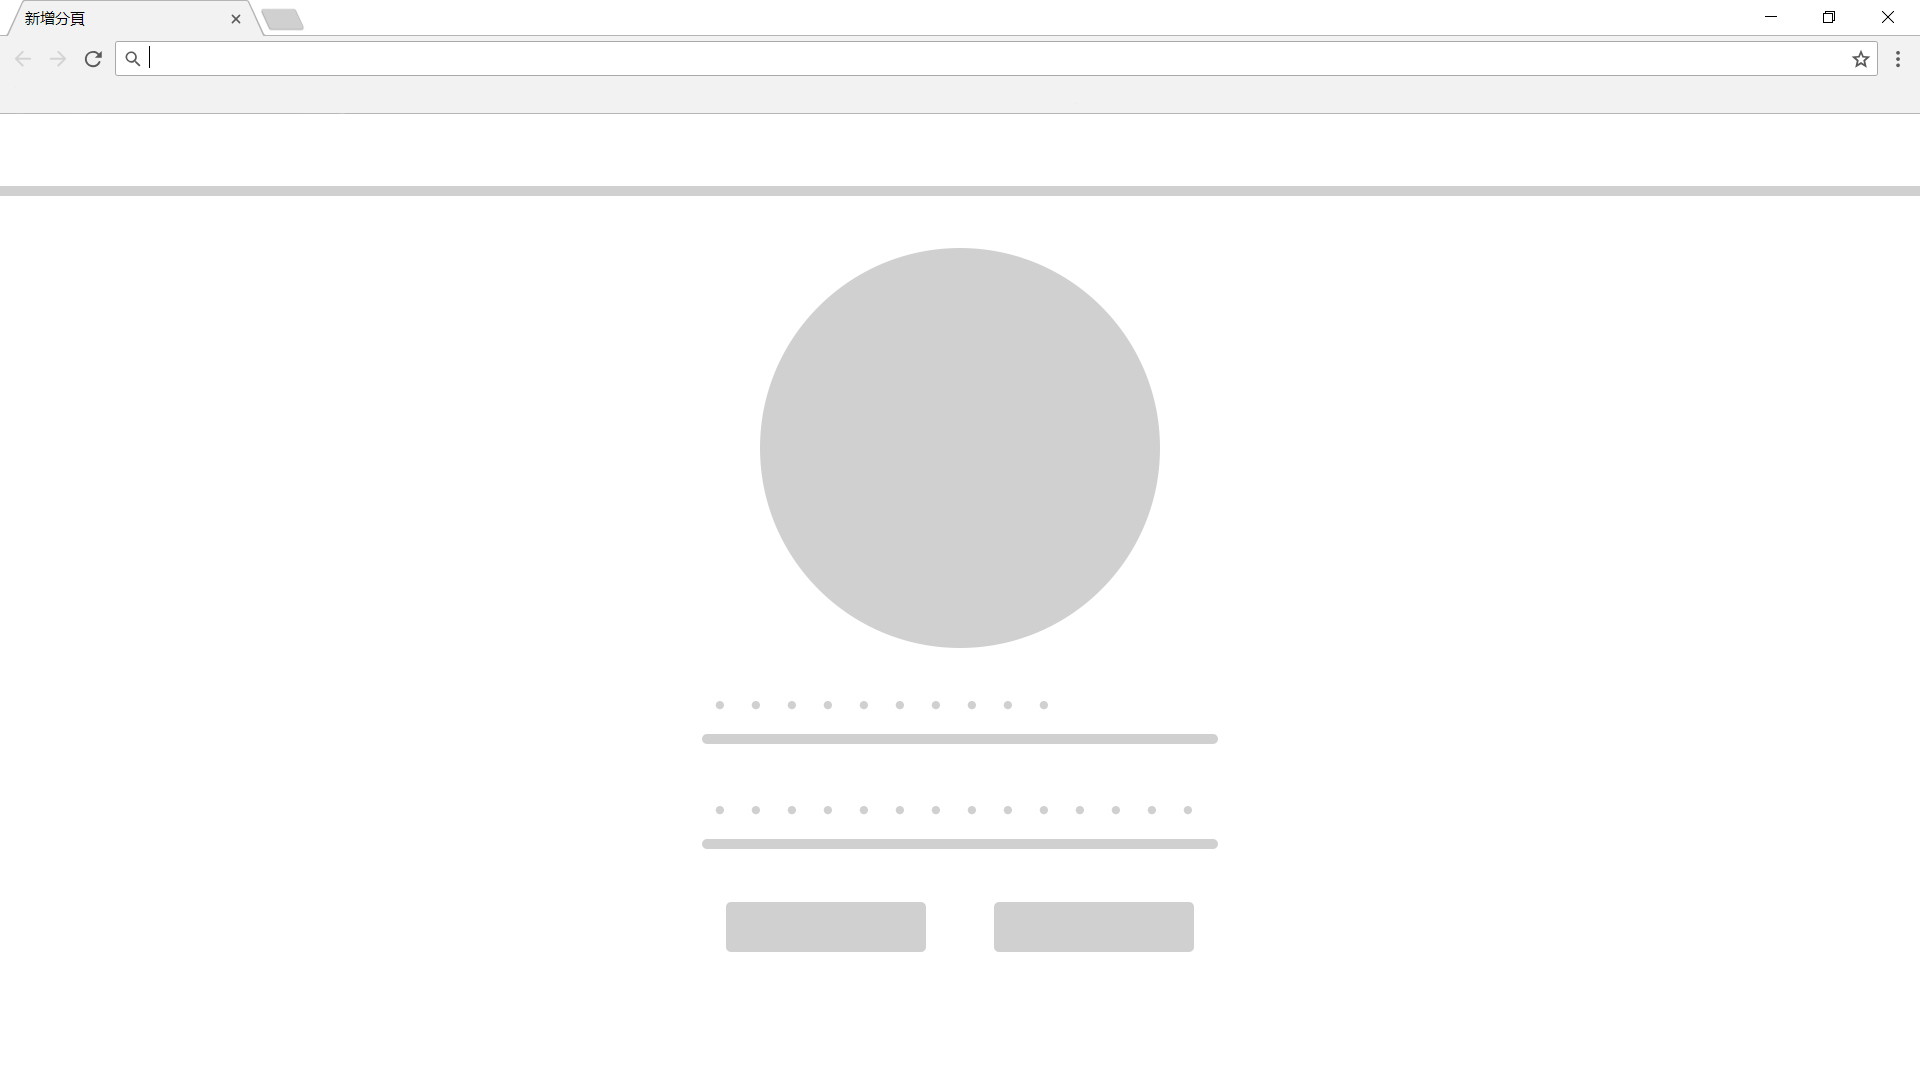
\includegraphics[width=16cm]{login.jpg}
\caption{用户登录界面示意图}\label{fig:noted-figure}
\end{figure}

\begin{figure}
\centering
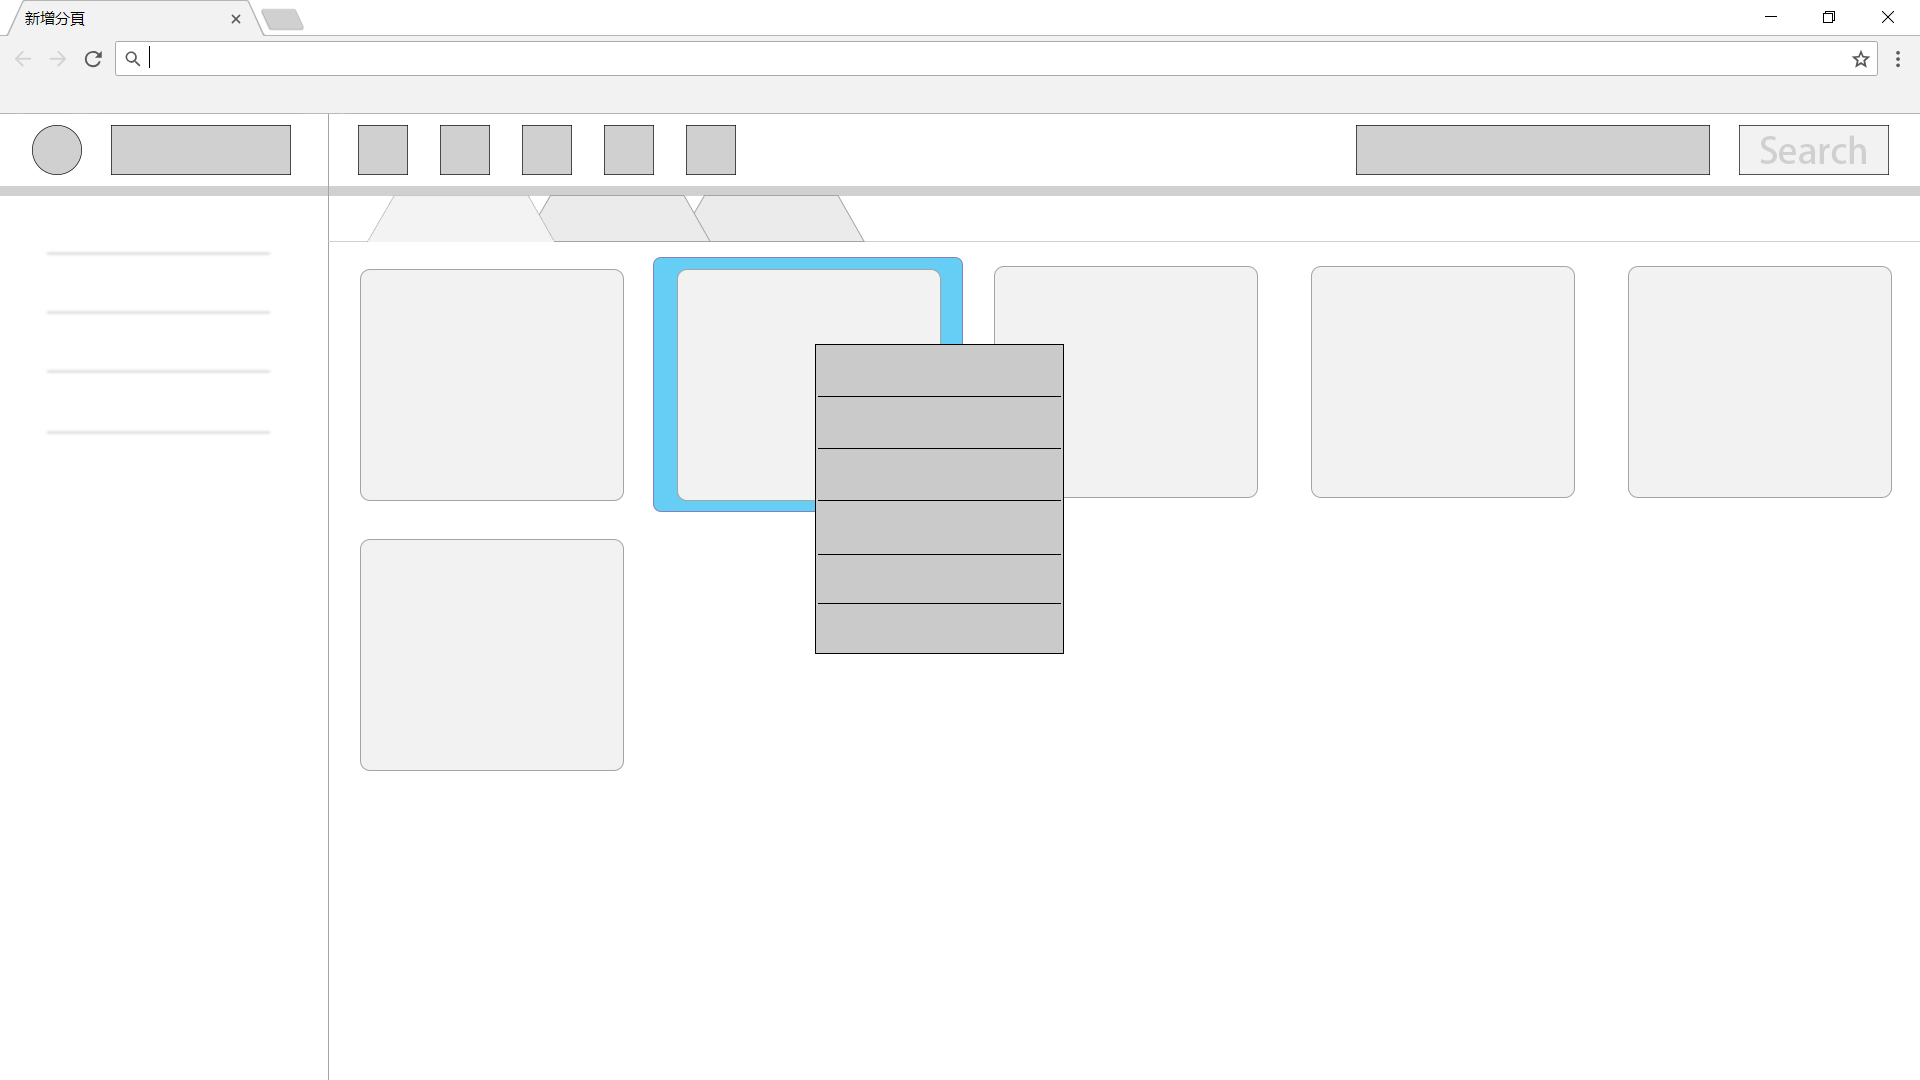
\includegraphics[width=16cm]{show.jpg}
\caption{右键界面示意图}\label{fig:noted-figure}
\end{figure}

\begin{figure}
\centering
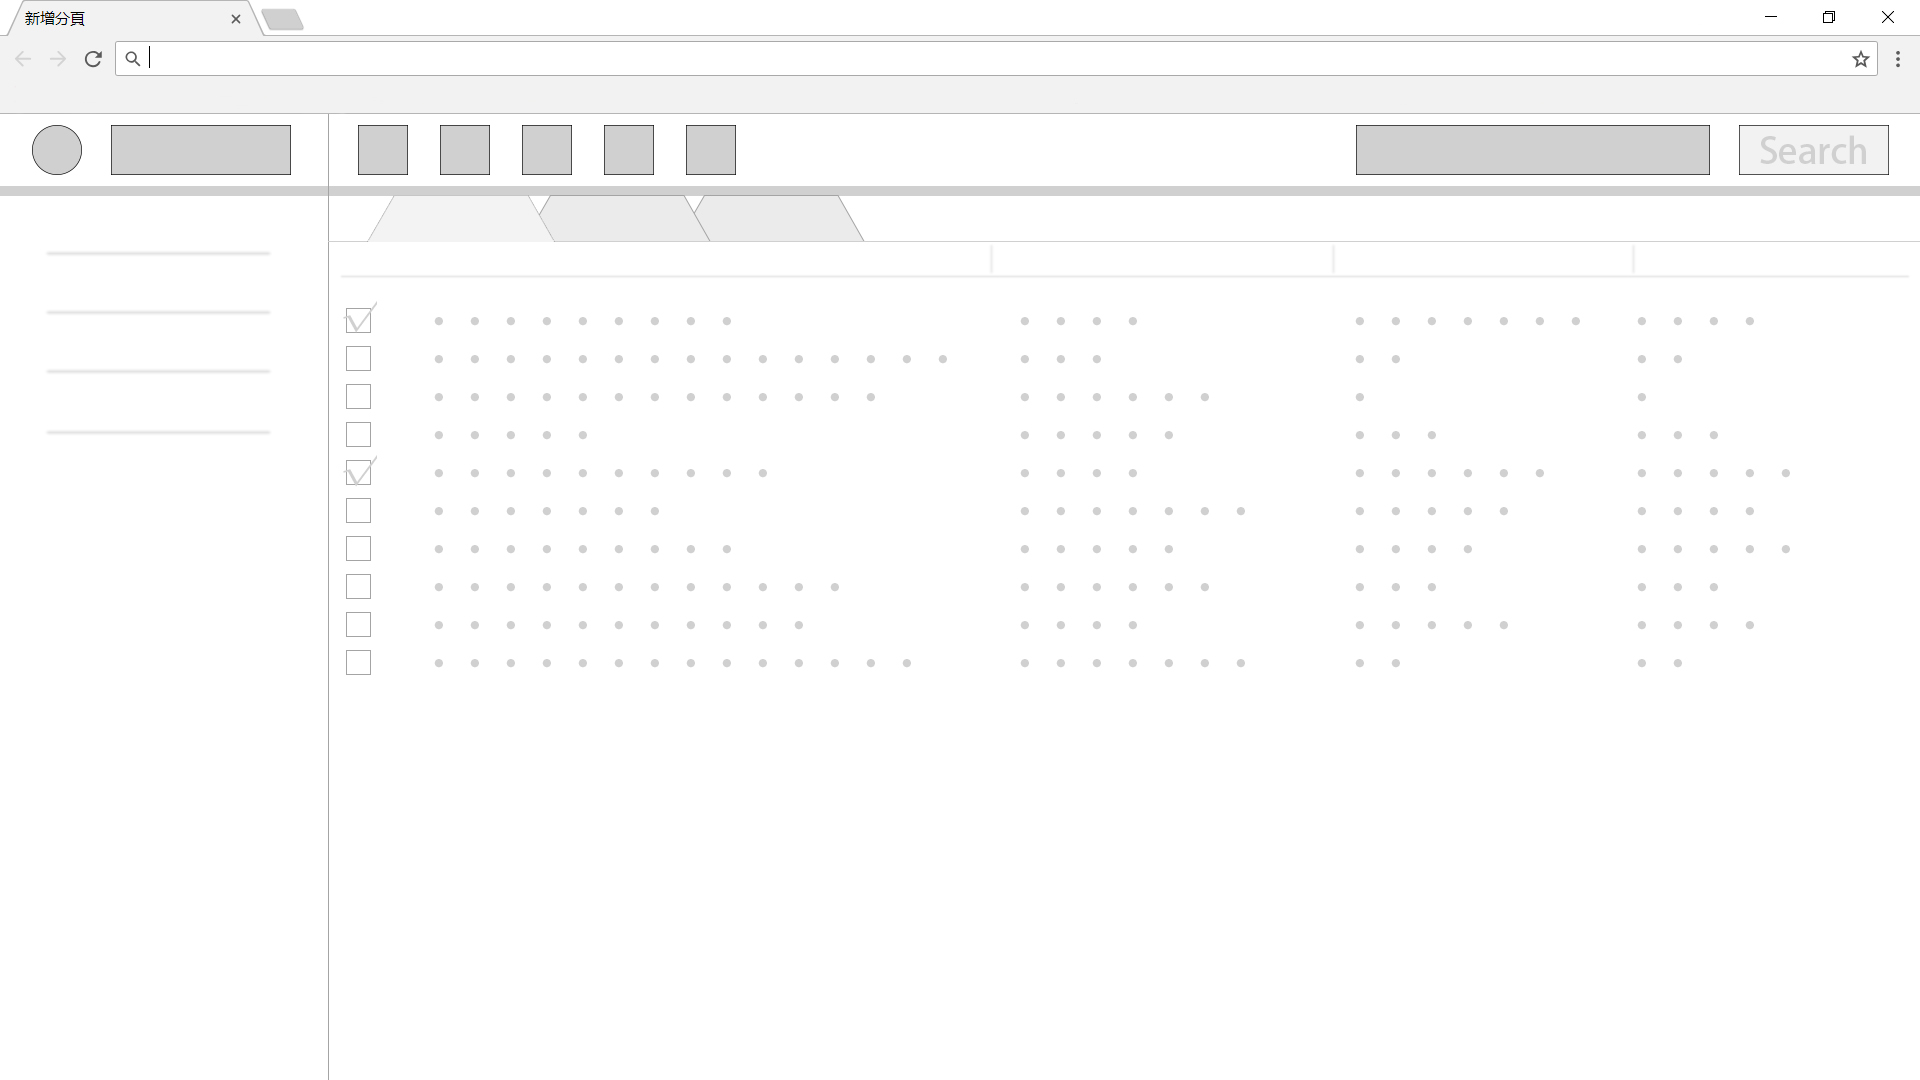
\includegraphics[width=16cm]{list.jpg}
\caption{列表显示示意图}\label{fig:noted-figure}
\end{figure}

\subsection{软件接口}

在此应描述如何使用其它(必需的)软件产品(例如,数据管理系统,操作系统,或算法工具包)
以及与其它应用系统的接口(例如,协议处理系统和数据库管理系统之间的接口)。

\subsubsection{数据管理系统}

名字:Mysql

助记符:Mysql

版本号:5

来源:官网

目的:服务器端的数据库服务,方便服务器端快速存取用户、文件等信息

\subsubsection{服务器操作系统}

名字:CentOS 

助记符:CentOS

版本号:7

来源:开源社区

目的:服务器端的运行环境,真个系统的支撑,方便开发人员进行开发、调试

\subsubsection{分布式文件系统}

名字:Ceph

助记符:Ceph 

版本号:12

来源:官网

目的:提供底层分布式的文件系统并实现高可用

\subsubsection{HTTP服务器}

名字:Tomcat

助记符:Tomcat

版本号: 9

来源: 官网

\subsubsection{后端框架语言}

名字:Java

助记符:Java

版本号:Java SE 10

来源:包管理器 

\subsection{硬件接口}

1. 服务器架构:x86/64的服务器主机集群或云主机

2. 服务器必须有1Gbps互联网接入

3. 服务器必须有100IOPS以上的磁盘(阵列)

\subsection{通讯接口}

与浏览器通讯:使用HTTP,HTTPS协议

参见 RFC2616、RFC2818、RFC2324 标准


